%
% A header that lets you compile a chapter by itself, or inside a larger document.
% Adapted from stackoverflow.com/questions/3655454/conditional-import-in-latex
%
%
%Use \inbpdocument and \outbpdocument in your individual files, in place of \begin{document} and \end{document}. In your main file, put in a \def \ismaindoc {} before including or importing anything.
%
% David Duvenaud
% June 2011
% 
% ======================================
%
%


\ifx\ismaindoc\undefined
	\newcommand{\inbpdocument}{
		\def \ismaindoc {}
		% Use this header if we are compiling by ourselves.
		\documentclass[a4paper,11pt,authoryear,index]{common/PhDThesisPSnPDF}
		
%\usepackage{draftwatermark}
%\SetWatermarkLightness{0.95}

% ******************************************************************************
% ****************************** Custom Margin *********************************

% Add `custommargin' in the document class options to use this section
% Set {innerside margin / outerside margin / topmargin / bottom margin}  and
% other page dimensions

\ifsetMargin
\else
    \RequirePackage[left=37mm,right=30mm,top=35mm,bottom=30mm]{geometry}
    \setFancyHdr % To apply fancy header after geometry package is loaded
\fi


%\chead{Unfinished draft}
%\cfoot{\texttt{Unfinished draft - compiled on \today{} at \currenttime}}

% *****************************************************************************
% ******************* Fonts (like different typewriter fonts etc.)*************

% Add `customfont' in the document class option to use this section

\ifsetFont
\else
    % Set your custom font here and use `customfont' in options. Leave empty to
    % load computer modern font (default LaTeX font).  

    \RequirePackage{libertine} 
\fi

% *****************************************************************************
% *************************** Bibliography  and References ********************

%\usepackage{cleveref} %Referencing without need to explicitly state fig /table

% Add `custombib' in the document class option to use this section
\ifsetBib % True, Bibliography option is chosen in class options
\else % If custom bibliography style chosen then load bibstyle here

   \RequirePackage[square, sort, numbers, authoryear]{natbib} % CustomBib

% If you would like to use biblatex for your reference management, as opposed to the default `natbibpackage` pass the option `custombib` in the document class. Comment out the previous line to make sure you don't load the natbib package. Uncomment the following lines and specify the location of references.bib file

% \RequirePackage[backend=biber, style=numeric-comp, citestyle=numeric, sorting=nty, natbib=true]{biblatex}
% \bibliography{References/references} %Location of references.bib only for biblatex

\fi


% changes the default name `Bibliography` -> `References'
\renewcommand{\bibname}{References}


% *****************************************************************************
% *************** Changing the Visual Style of Chapter Headings ***************
% Uncomment the section below. Requires titlesec package.

%\RequirePackage{titlesec}
%\newcommand{\PreContentTitleFormat}{\titleformat{\chapter}[display]{\scshape\Large}
%{\Large\filleft{\chaptertitlename} \Huge\thechapter}
%{1ex}{}
%[\vspace{1ex}\titlerule]}
%\newcommand{\ContentTitleFormat}{\titleformat{\chapter}[display]{\scshape\huge}
%{\Large\filleft{\chaptertitlename} \Huge\thechapter}{1ex}
%{\titlerule\vspace{1ex}\filright}
%[\vspace{1ex}\titlerule]}
%\newcommand{\PostContentTitleFormat}{\PreContentTitleFormat}
%\PreContentTitleFormat


% *****************************************************************************
% **************************** Custom Packages ********************************
% *****************************************************************************


% ************************* Algorithms and Pseudocode **************************

%\usepackage{algpseudocode} 


% ********************Captions and Hyperreferencing / URL **********************

% Captions: This makes captions of figures use a boldfaced small font. 
%\RequirePackage[small,bf]{caption}

\RequirePackage[labelsep=space,tableposition=top]{caption} 
%\renewcommand{\figurename}{Figure} %to support older versions of captions.sty
\captionsetup{labelsep = colon,belowskip=12pt,aboveskip=4pt}

% ************************ Formatting / Footnote *******************************

%\usepackage[perpage]{footmisc} %Range of footnote options 


% ****************************** Line Numbers **********************************

%\RequirePackage{lineno}
%\linenumbers

% ************************** Graphics and figures *****************************

%\usepackage{rotating}
%\usepackage{wrapfig}
%\usepackage{float}
\usepackage{subfig} %note: subfig must be included after the `caption` package. 


% ********************************* Table **************************************

%\usepackage{longtable}
%\usepackage{multicol}
%\usepackage{multirow}
%\usepackage{tabularx}


% ***************************** Math and SI Units ******************************

\usepackage{amsfonts}
\usepackage{amsmath}
\usepackage{amssymb}
%\usepackage{siunitx} % use this package module for SI units


% ******************************************************************************
% ************************* User Defined Commands ******************************
% ******************************************************************************

% *********** To change the name of Table of Contents / LOF and LOT ************

%\renewcommand{\contentsname}{My Table of Contents}
%\renewcommand{\listfigurename}{List of figures}
%\renewcommand{\listtablename}{List of tables}


% ********************** TOC depth and numbering depth *************************

\setcounter{secnumdepth}{2}
\setcounter{tocdepth}{2}

% ******************************* Nomenclature *********************************

% To change the name of the Nomenclature section, uncomment the following line

%\renewcommand{\nomname}{Symbols}


% ********************************* Appendix ***********************************

% The default value of both \appendixtocname and \appendixpagename is `Appendices'. These names can all be changed via: 

%\renewcommand{\appendixtocname}{List of appendices}
%\renewcommand{\appendixname}{Appndx}

		% All my custom preamble stuff.  Shouldn't overlap with anything in official-preamble




% Paths to figure and table directories.
\newcommand{\symmetryfigsdir}{figures/symmetries}
\newcommand{\topologyfiguresdir}{figures/topology}
\newcommand{\infinitefiguresdir}{figures/infinite}
\newcommand{\grammarfiguresdir}{figures/grammar}
\newcommand{\introfigsdir}{figures/intro}
\newcommand{\gplvmfiguresdir}{figures/gplvm}
\newcommand{\warpedfiguresdir}{figures/warped-mixtures}
\newcommand{\deeplimitsfiguresdir}{figures/deep-limits}
\newcommand{\quadraturefigsdir}{figures/quadrature}
\newcommand{\additivefigsdir}{figures/additive}
\newcommand{\decompfigsdir}{figures/decomp}
\newcommand{\examplefigsdir}{figures/worked-example}

\usepackage{bm}  % for warped mixtures - is this necessary?
\usepackage{booktabs}
\usepackage{tabularx}
\usepackage{multirow}
\usepackage{datetime}
\renewcommand{\tabularxcolumn}[1]{>{\arraybackslash}m{#1}}
\usepackage{relsize}
\usepackage{graphicx}
\usepackage{amsmath,amssymb,textcomp}
\usepackage{nicefrac}
\usepackage{amsthm}
\usepackage{tikz}
\usetikzlibrary{arrows}
\usetikzlibrary{calc}
\usepackage{nth}
\usepackage{rotating}
\usepackage{array}
\usepackage{fp}
\usepackage{cleveref}   % Note: this package sometimes causes the page counter to reset.
\crefname{equation}{equation}{equations}
\crefname{figure}{figure}{figures}
%\usepackage{common/sectsty}

% Controls capitalization of all headers
%\usepackage{stringstrings}
%\usepackage[explicit]{titlesec}
%\newcommand\SentenceCase[1]{%
%  \caselower[e]{#1}%
%  \capitalize[q]{\thestring}%
%}
%\titleformat{\section}
%  {\normalfont\Large\bfseries}{\thesection}{1em}{\SentenceCase{#1}\thestring}


%\titleformat{\section} % The normal, unstarred version
%    {\Large\bfseries}{}{2ex}
%    {\thesection. \MakeSentenceCase{#1}}

%\titleformat{name=\section,numberless} % The starred version; note the `numberless` key
%    {\Large\bfseries}{}{2ex}
%    {\MakeSentenceCase{#1}}

\usepackage[hyperpageref]{backref}
% Setup to show (pages 4 and 9) sort of thing in the bibliography - DD
%\def\foo{\hspace{\fill}\mbox{}\linebreak[0]\hspace*{\fill}}
%\def\foo{\parbox{3cm}{\hfill}
%\def\foo{\parbox{3cm}{\hfill}
%\newcommand\foo[1]{{\raggedleft{\hfill{\mbox{\hfill{#1}}}}}}
\newcommand{\comfyfill}[1]{% = Thorsten Donig's \signed
  \unskip\hspace*{0.1em plus 1fill}
  \nolinebreak[3]%
  \hspace*{\fill}\mbox{#1}
  \parfillskip0pt\par
}
\newcommand\foo[1]{{\comfyfill{\mbox{#1}}}}
%\newcommand\foo[1]{{\mbox{#1}}}
\renewcommand*{\backref}[1]{}
\renewcommand*{\backrefalt}[4]{%
\ifcase #1 %
%
\or
\foo{(page #2)}%
\else
\foo{(pages #2)}%
\fi
}

\usepackage{stringstrings}

%\newcommand{\headercase}{\
%\DeclareFieldFormat{titlecase}{\MakeSentenceCase{#1}}


%% For submission, make all render blank.
%%%%%%%%%%%%%%%%%%%%%%%%%%%%%%%%%%%%%%%%%%%%%%%%%%%%%%%%%%
%%%% EDITING HELPER FUNCTIONS  %%%%%%%%%%%%%%%%%%%%%%%%%%%
%%%%%%%%%%%%%%%%%%%%%%%%%%%%%%%%%%%%%%%%%%%%%%%%%%%%%%%%%%

%% NA: needs attention (rough writing whose correctness needs to be verified)
%% TBD: instructions for how to fix a gap ("Describe the propagation by ...")
%% PROBLEM: bug or missing crucial bit 

%% use \fXXX versions of these macros to put additional explanation into a footnote.  
%% The idea is that we don't want to interrupt the flow of the paper or make it 
%% impossible to read because there are a bunch of comments.

%% NA's (and TBDs, those less crucially) should be written so 
%% that they flow with the text.

\definecolor{WowColor}{rgb}{.75,0,.75}
\definecolor{SubtleColor}{rgb}{0,0,.50}

% inline
\newcommand{\NA}[1]{\textcolor{SubtleColor}{ {\tiny \bf ($\star$)} #1}}
\newcommand{\LATER}[1]{\textcolor{SubtleColor}{ {\tiny \bf ($\dagger$)} #1}}
\newcommand{\TBD}[1]{\textcolor{SubtleColor}{ {\tiny \bf (!)} #1}}
\newcommand{\PROBLEM}[1]{\textcolor{WowColor}{ {\bf (!!)} {\bf #1}}}

% as margin notes

\newcounter{margincounter}
\newcommand{\displaycounter}{{\arabic{margincounter}}}
\newcommand{\incdisplaycounter}{{\stepcounter{margincounter}\arabic{margincounter}}}

\newcommand{\fTBD}[1]{\textcolor{SubtleColor}{$\,^{(\incdisplaycounter)}$}\marginpar{\tiny\textcolor{SubtleColor}{ {\tiny $(\displaycounter)$} #1}}}

\newcommand{\fPROBLEM}[1]{\textcolor{WowColor}{$\,^{((\incdisplaycounter))}$}\marginpar{\tiny\textcolor{WowColor}{ {\bf $\mathbf{((\displaycounter))}$} {\bf #1}}}}

\newcommand{\fLATER}[1]{\textcolor{SubtleColor}{$\,^{(\incdisplaycounter\dagger)}$}\marginpar{\tiny\textcolor{SubtleColor}{ {\tiny $(\displaycounter\dagger)$} #1}}}

%\renewcommand{\LATER}[1]{}
%\renewcommand{\fLATER}[1]{}
%\renewcommand{\TBD}[1]{}
%\renewcommand{\fTBD}[1]{}
%\renewcommand{\PROBLEM}[1]{}
%\renewcommand{\fPROBLEM}[1]{}
%\renewcommand{\NA}[1]{}


% HUMBLE WORDS: shown slightly smaller when in normal text
% Thanks to Christian Steinruecken!

% HUMBLE WORDS: shown slightly smaller when in normal text
% Christian Steinruecken
%
\makeatletter%
%\def\@humbleformat#1{{\fontsize{}{1em}\selectfont #1}}
%\def\@humbleformat#1{\textsmaller{#1}}%
\newlength{\nonHumbleHeight}
\def\@humbleformat#1{{\settoheight{\nonHumbleHeight}{#1}\resizebox{!}{0.94\nonHumbleHeight}{#1}}}%
\def\@idxhumbleformat#1{{\relscale{0.95}{#1}}}%
%\def\@humbleformat#1{{#1}}%
\def\declareHumble#1#2{%
  \expandafter\def\csname #1\endcsname{\@humbleformat{#2}}%
  \expandafter\def\csname s#1\endcsname{{#2}}%
  \expandafter\def\csname idx#1\endcsname{{\@idxhumbleformat{#2}}}%
}%
\def\humble#1{\@humbleformat{#1}}%
\def\idxhumble#1{\@idxhumbleformat{#1}}%
\makeatother%

% Convenient indexing for humble abbreviations
\def\humbleindex#1#2{\index{#1@\idxhumble{#1}}}



% TODO: Clean up duplicates
\declareHumble{ANOVA}{ANOVA}
\declareHumble{ARD}{ARD}
\declareHumble{BIC}{BIC}
\declareHumble{BMC}{BMC}
\declareHumble{bq}{BQ}
\declareHumble{CRP}{CRP}
\declareHumble{dirpro}{DP}
\declareHumble{HDMR}{HDMR}
\declareHumble{GAM}{GAM}
\declareHumble{GEM}{GEM}
\declareHumble{GMM}{GMM}
\declareHumble{gplvm}{GP-LVM}
\declareHumble{gpml}{GPML}
\declareHumble{GPML}{GPML}
\declareHumble{gprn}{GPRN}
\declareHumble{gpt}{GP}
\declareHumble{gp}{GP}
\declareHumble{HKL}{HKL}
\declareHumble{HMC}{HMC}
\declareHumble{ibp}{IBP}
\declareHumble{iGMM}{iGMM}
\declareHumble{iwmm}{iWMM}
\declareHumble{kCP}{CP}
\declareHumble{kCW}{CW}
\declareHumble{kC}{C}
\declareHumble{KDE}{KDE}
\declareHumble{kLin}{Lin}
\declareHumble{KPCA}{KPCA}
\declareHumble{kPer}{Per}
\declareHumble{kPerGen}{ZMPer}
\declareHumble{kRQ}{RQ}
\declareHumble{kSE}{SE}
\declareHumble{kWN}{WN}
\declareHumble{Lin}{Lin}
\declareHumble{LBFGS}{L-BFGS}
\declareHumble{LIBSVM}{LIBSVM}
\declareHumble{MAP}{MAP}
\declareHumble{mcmc}{MCMC}
\declareHumble{MKL}{MKL}
\declareHumble{MLP}{MLP}
\declareHumble{MNIST}{MNIST}
\declareHumble{MSE}{MSE}
\declareHumble{OU}{OU}
\declareHumble{Per}{Per}
\declareHumble{RBF}{RBF}
\declareHumble{RMSE}{RMSE}
\declareHumble{RQ}{RQ}
\declareHumble{SBQ}{SBQ}
\declareHumble{seard}{SE-ARD}
\declareHumble{sefull}{SE-\textnormal{full}}
\declareHumble{SEGP}{SE-GP}
\declareHumble{SE}{SE}
\declareHumble{SNR}{SNR}
\declareHumble{SSANOVA}{SS-ANOVA}
\declareHumble{SVM}{SVM}
\declareHumble{UCI}{UCI}
\declareHumble{UMIST}{UMIST}
\declareHumble{vbgplvm}{VB GP-LVM}

\newcommand{\kSig}{\boldsymbol\sigma}

\def\subexpr{{\cal S}}
\def\baseker{{\cal B}}
\def\numWinners{k}

\def\ie{i.e.\ }
\def\eg{e.g.\ }
\def\etc{etc.\ }
\let\oldemptyset\emptyset
%\let\emptyset 0




% Unify notation between neural-net land and GP-land.
\newcommand{\hphi}{h}
\newcommand{\hPhi}{\vh}
\newcommand{\walpha}{w}
\newcommand{\wboldalpha}{\bw}
\newcommand{\wcapalpha}{\vW}
\newcommand{\lengthscale}{w}

\newcommand{\layerindex}{\ell}



\newcommand{\gpdrawbox}[1]{
\setlength\fboxsep{0pt}
\hspace{-0.15in} 
\fbox{
\includegraphics[width=0.464\columnwidth]{\deeplimitsfiguresdir/deep_draws/deep_gp_sample_layer_#1}
}}



\newcommand{\procedurename}{ABCD}
\newcommand{\genText}[1]{{\sf #1}}



\newcommand{\asdf}{$^{\textnormal{th}}$}

\newcommand{\binarysum}{\sum_{\bf{x} \in \{0,1\}^D}}
\newcommand{\expect}{\mathbb{E}}
\newcommand{\expectargs}[2]{\mathbb{E}_{#1} \left[ {#2} \right]}
\newcommand{\var}{\mathbb{V}}
\newcommand{\varianceargs}[2]{\mathbb{V}_{#1} \left[ {#2} \right]}
\newcommand{\cov}{\operatorname{cov}}
\newcommand{\Cov}{\operatorname{Cov}}
\newcommand{\covargs}[2]{\Cov \left[ {#1}, {#2} \right]}
\newcommand{\variance}{\mathbb{V}}
\newcommand{\vecop}[1]{\operatorname{vec} \left( {#1} \right)}

\newcommand{\covarianceargs}[2]{\Cov_{#1} \left[ {#2} \right]}
\newcommand{\colvec}[2]{\left[ \begin{array}{c} {#1} \\ {#2} \end{array} \right]}
\newcommand{\tbtmat}[4]{\left[ \begin{array}{cc} {#1} & {#2} \\ {#3} & {#4} \end{array} \right]}

\newcommand{\acro}[1]{{\humble{#1}}}
%\newcommand{\vect}[1]{\boldsymbol{#1}}
\newcommand{\vect}[1]{{\bf{#1}}}
\newcommand{\mat}[1]{\mathbf{#1}}
\newcommand{\pderiv}[2]{\frac{\partial #1}{\partial #2}}
\newcommand{\npderiv}[2]{\nicefrac{\partial #1}{\partial #2}}

\newcommand{\pha}{^{\phantom{:}}}

\newcommand{\argmin}{\operatornamewithlimits{argmin}}
\newcommand{\argmax}{\operatornamewithlimits{argmax}}

% The following designed for probabilities with long arguments

\newcommand{\Prob}[2]{P\!\left(\,#1\;\middle\vert\;#2\,\right)}
\newcommand{\ProbF}[3]{P\!\left(\,#1\!=\!#2\;\middle\vert\;#3\,\right)}
\newcommand{\p}[2]{p\!\left(#1\middle\vert#2\right)}
\newcommand{\po}[1]{p\!\left(#1\right)}
\newcommand{\pF}[3]{p\!\left(\,#1\!=\!#2\;\middle\vert\;#3\,\right)} 
\newcommand{\mean}[2]{{m}\!\left(#1\middle\vert#2\right)}



\newcommand{\valpha}{\boldsymbol{\alpha}}
\newcommand{\va}{\vect{a}}
\newcommand{\vA}{\vect{A}}
\newcommand{\vB}{\mat{B}}
\newcommand{\vb}{\vect{b}}
\newcommand{\vC}{\mat{C}}
\newcommand{\vc}{\vect{c}}
\newcommand{\vecf}{\boldsymbol{f}}
\newcommand{\vell}{\vect{\ell}}
\newcommand{\vepsilon}{\boldsymbol{\epsilon}}
\newcommand{\veps}{\boldsymbol{\epsilon}}
\newcommand{\ve}{\boldsymbol{\epsilon}}
\newcommand{\vf}{\vecf}
\newcommand{\vg}{\vect{g}}
\newcommand{\vh}{\vect{h}}
\newcommand{\vI}{\mat{I}}
\newcommand{\vK}{\mat{K}}
\newcommand{\vk}{\vect{k}}
\newcommand{\vL}{\mat{L}}
\newcommand{\vl}{\vect{l}}
\newcommand{\vmu}{{\boldsymbol{\mu}}}
\newcommand{\vone}{\vect{1}}
\newcommand{\vphi}{{\boldsymbol{\phi}}}
\newcommand{\vpi}{{\boldsymbol{\pi}}}
\newcommand{\vq}{\vect{q}}
\newcommand{\vR}{\mat{R}}
\newcommand{\vr}{\vect{r}}
\newcommand{\vsigma}{{\boldsymbol{\sigma}}}
\newcommand{\vSigma}{\mat{\Sigma}}
\newcommand{\vS}{\mat{S}}
\newcommand{\vs}{\vect{s}}
\newcommand{\vtheta}{{\boldsymbol{\theta}}}
\newcommand{\vu}{\vect{u}}
\newcommand{\vV}{\mat{V}}
\newcommand{\vW}{\mat{W}}
\newcommand{\vw}{\vect{w}}
\newcommand{\vX}{\mat{X}}
\newcommand{\vx}{\vect{x}}
\newcommand{\vY}{\mat{Y}}
\newcommand{\vy}{\vect{y}}
\newcommand{\vzero}{\vect{0}}
\newcommand{\vZ}{\mat{Z}}
\newcommand{\vz}{\vect{z}}


% deep gp notation
\newcommand{\netweights}{w}
\newcommand{\vnetweights}{\vw}
\newcommand{\mnetweights}{\vW}
\newcommand{\outweights}{\v}
\newcommand{\voutweights}{\vv}
\newcommand{\moutweights}{\vV}

\newcommand{\unitparams}{\v}
\newcommand{\vunitparams}{\vv}
\newcommand{\munitparams}{\vV}


\newcommand{\He}{\mathcal{H}}
\newcommand{\normx}[2]{\left\|#1\right\|_{#2}}
\newcommand{\Hnorm}[1]{\normx{#1}{\He}}
\newcommand{\mmd}{{\rm MMD}}


\newcommand{\mf}{\bar{\vf}}

%\newcommand{\mf}{\mu} %{\bar{\ell}}
\newcommand{\lf}{f} % Likelihood function
\newcommand{\st}{_\star}

% from simpler log-bq writeup
\newcommand{\lftwo}{{\log \ell}}
\newcommand{\mftwo}{{\bar \ell}}
\newcommand{\loggp}{{\log\acro{GP}}}%| \bX, \vy )}}
\newcommand{\loggpdist}{{\acro{GP}(\lftwo)}}%| \vX, \vy )}}


\newcommand{\inv}{^{{\mathsmaller{-1}}}}
\newcommand{\tohalf}{^{{\mathsmaller{\nicefrac{1}{2}}}}}

\newcommand{\Normal}{\mathcal{N}}
\newcommand{\N}[3]{\mathcal{N}\!\left(#1 \middle| #2,#3\right)}
\newcommand{\Nt}[2]{\mathcal{N}\!\left(#1,#2\right)}
\newcommand{\NT}[2]{\mathcal{N}\!\left(#1,#2\right)}
\newcommand{\GPdist}[3]{\mathcal{GP}\!\left(#1 \, \middle| \, #2, #3 \right)}
\newcommand{\GPdisttwo}[2]{\mathcal{GP}\!\left(\, #1, #2 \right)}
\newcommand{\bN}[3]{\mathcal{N}\big(#1 \middle| #2,#3\big)}
\newcommand{\boldN}[3]{\text{\textbf{\mathcal{N}}}\big(#1;#2,#3\big)}
\newcommand{\ones}[1]{\mat{1}_{#1}}
\newcommand{\eye}[1]{\mat{E}_{#1}}
\newcommand{\tra}{^{\mathsf{T}}}
%\newcommand{\tra}{^{\top}}
%\mathsf{T}
\newcommand{\trace}{\operatorname{tr}}
\newcommand{\shift}{\operatorname{shift}}
\renewcommand{\mod}{\operatorname{mod}}
\newcommand{\deq}{:=}
\newcommand{\oneofk}{\operatorname{one-of-k}}
%\newcommand{\degree}{^\circ}

\newcommand{\GPt}[2]{\mathcal{GP}\!\left(#1,#2\right)}
%\newcommand{\GPt}[2]{\gp\!\left(#1,#2\right)}

\DeclareMathOperator{\tr}{tr}
\DeclareMathOperator{\chol}{chol}
\DeclareMathOperator{\diag}{diag}

\newenvironment{narrow}[2]{%
  \begin{list}{}{%
  \setlength{\topsep}{0pt}%
  \setlength{\leftmargin}{#1}%
  \setlength{\rightmargin}{#2}%
  \setlength{\listparindent}{\parindent}%
  \setlength{\itemindent}{\parindent}%
  \setlength{\parsep}{\parskip}}%
\item[]}{\end{list}}



\newcommand{\dist}{\ \sim\ }
\def\given{\,|\,}

% Table stuff
\newcolumntype{C}[1]{>{\centering\let\newline\\\arraybackslash\hspace{0pt}}m{#1}}
\newcolumntype{L}[1]{>{\raggedright\let\newline\\\arraybackslash\hspace{0pt}}m{#1}}
\newcolumntype{R}[1]{>{\raggedleft\let\newline\\\arraybackslash\hspace{0pt}}m{#1}}

\newcommand{\defeq}{\mathrel{:\mkern-0.25mu=}}

\def\ie{i.e.\ }
\def\eg{e.g.\ }
\def\iid{i.i.d.\ }
%\def\simiid{\sim_{\mbox{\tiny iid}}}
\def\simiid{\overset{\mbox{\tiny iid}}{\sim}}
\def\simind{\overset{\mbox{\tiny \textnormal{ind}}}{\sim}}
\def\eqdist{\stackrel{\mbox{\tiny d}}{=}}
%\newcommand{\distas}[1]{\mathbin{\overset{#1}{\kern \z@ \sim}}}
%TODO: fix this - it worked outside the thesis!
\newcommand{\distas}[1]{\mathbin{\overset{#1}{\sim}}}

\def\Reals{\mathbb{R}}

\def\Uniform{\mbox{\rm Uniform}}
\def\Bernoulli{\mbox{\rm Bernoulli}}
\def\GP{\mathcal{GP}}
\def\GPLVM{\mathcal{GP-LVM}}




% Kernel stuff

\def\iva{\vect{\inputVar}}
\def\ivaone{\inputVar}
\def\inputVar{x}
\def\InputVar{X}
\def\InputSpace{\mathcal{X}}
\def\outputVar{y}
\def\OutputSpace{\mathcal{Y}}
\def\function{f}
\def\kernel{k}
\def\KernelMatrix{K}
\def\SumKernel{\sum}
\def\ProductKernel{\prod}
\def\expression{e}
\def\feat{\vh}

\newcommand{\kerntimes}{ \! \times \!}
\newcommand{\kernplus}{ \, + \,}


% Proof stuff
\theoremstyle{plain}
\newtheorem{theorem}{Theorem}[section]
\newtheorem{lemma}[theorem]{Lemma}
\newtheorem{prop}[theorem]{Proposition}
\newtheorem{proposition}{Proposition}
\newtheorem*{cor}{Corollary}

% For infinite bq
\newcommand{\iv}{\theta}
\newcommand{\viv}{\vtheta}

% For intro chapter
\newcommand{\funcval}{\vf(\vX)}
\newcommand{\testpoint}{{\vx^\star}}

\newcommand{\underwrite}[2]{{\underbrace{#1}_{\textnormal{#2}}}}



% For kernel figures
\newcommand{\fhbig}{2cm}%
\newcommand{\fwbig}{3cm}%
\newcommand{\kernpic}[1]{\includegraphics[height=\fhbig,width=\fwbig]{\grammarfiguresdir/structure_examples/#1}}%
\newcommand{\kernpicr}[1]{\rotatebox{90}{\includegraphics[height=\fwbig,width=\fhbig]{\grammarfiguresdir/structure_examples/#1}}}%
\newcommand{\addkernpic}[1]{{\includegraphics[height=\fhbig,width=\fwbig]{\grammarfiguresdir/additive_multi_d/#1}}}%
\newcommand{\largeplus}{\tabbox{{\Large+}}}%
\newcommand{\largeeq}{\tabbox{{\Large=}}}%
\newcommand{\largetimes}{\tabbox{{\Large$\times$}}}%
\newcommand{\fixedx}{$x$ (with $x' = 1$)}%

% for warped mixtures
\newcommand{\CLAS}{\vz}  %cluster assignments
\newcommand{\CLASi}{z} % individual cluster assignments


		% ************************ Thesis Information & Meta-data **********************

%% The title of the thesis
\title{Automating statistical modelling}

%\texorpdfstring is used for PDF metadata. Usage:
%\texorpdfstring{LaTeX_Version}{PDF Version (non-latex)} eg.,
%\texorpdfstring{$sigma$}{sigma}

%% The full name of the author
\author{James Robert Lloyd}

%% Department (eg. Department of Engineering, Maths, Physics)
%\dept{Department of Engineering}

%% University and Crest
\university{University of Cambridge}
\crest{
\includegraphics[width=0.25\textwidth]{misc/University_Crest}}

%% You can redefine the submission text:
% Default as per the University guidelines: This dissertation is submitted for
% the degree of Doctor of Philosophy
%\renewcommand{\submissiontext}{change the default text here if needed}

%% Full title of the Degree 
\degree{Doctor of Philosophy}
 
%% College affiliation (optional)
\college{Trinity College}

%% Submission date
\degreedate{December 2014} 

%% Meta information
\subject{Machine Learning}
\keywords{{LaTeX} {PhD Thesis} {Engineering} {University of Cambridge} {Machine Learning} {Gaussian processes} {Time Series} {Model checking} {Model criticism} {Aldous--Hoover} {Networks}}



		\begin{document}
	}	
	\newcommand{\outbpdocument}[1]{
		% Fake chapters so references aren't broken
		\label{ch:intro}                
		\label{ch:dummy}
		\label{ch:discussion}
		%\bibliographystyle{common/CUEDthesis}
		\bibliographystyle{plainnat}
		\bibliography{references.bib}
		\end{document}
	}	
\else
	%If we're inside another document, no need to re-start the document.
	\ifx\inbpdocument\undefined
		\newcommand{\inbpdocument}{}
		\newcommand{\outbpdocument}[1]{}
	\fi
\fi

\inbpdocument

\chapter{Representing probability distributions of exchangeable arrays}
\label{ch:arrays}

In chapter~\ref{ch:networks} we demonstrated how to characterise probability distributions over objects such as networks or user--item rating matrices.
The key properties that allowed us to characterise these distributions were symmetries in the data, or invariances to the way they are stored.
For networks, we assumed that the ordering of the nodes contained no information.
For user--item data we assumed that the order of both users and items were irrelevant to the meaning of the data.

In this chapter we extend these ideas of exchangeability to any data that can be stored in a relational database.
We demonstrate that extensions of the \NA{Aldous--Hoover} theorem to $n$-arrays due to Kallenberg \NA{cite} can be extended to the case of exchangeable databases.
These new theorems reveal a natural parameter space for data stored in relational databases elucidating how to construct appropriate statistical models for such data.

This chapter is largely based on collaborations with Zoubin Ghahramani, Peter Orbanz and Daniel Roy.
In particular, the theorems presented in this chapter appeared at \NA{BNP} and \NA{NIPS} workshops but without proof.

\section{Introduction}

Relational databases are an extremely common data structure so it is natural to want to perform statistical tasks with such data \eg predicting unobserved data or identifying latent structure.
In particular, network data is rarely encountered in isolation \eg in a social network one will often have access to side information about each user.
To perform a statistical analysis of such data we will typically need to estimate parameters of a probabilistic model, but it is not immediately clear what an appropriate parameter space for such a model is.
The choice of parameter space is important because it indicates the targets of statistical inference and shows where we can share statistical strength between different aspects of the data.

We demonstrate that the weak assumption of an appropriate form of exchangeability can provide a natural parameter space.
%Exchangeability is a reasonable assumption whenever we can faithfully model our data as being a random finite sample from some theoretical infinite population where the order of sampling does not matter.
This form of exchangeability is appropriate when the order of the objects underlying a relational database (\eg users and movies in a database of ratings data) is arbitrary or unimportant.
For example, the left hand side of figure~\ref{fig:exchangeable} shows the same network but with differently labeled nodes.
If the labeling is unimportant, then any probabilistic model of such data should assign them the same probability.

\begin{figure}[t]
\centering
\begin{tabular}{c}
\tiny \begin{tikzpicture}[scale=3]
  \begin{scope}[yshift=0cm]
    \tikzstyle{graph_node}=[circle,minimum size=0.0225\textwidth,inner sep=0pt, fill=camlightblue]
    \def \radius {0.0225\textwidth}
    \begin{scope}[xshift=0cm]
      \foreach \s in {1,...,10}
      {
        \node[draw, graph_node] (N\s) at ({360/10 * (\s - 1) + 90}:\radius) {\s};
      }   
      \path (N2) edge (N6);
      \path (N4) edge (N9);
      \path (N5) edge (N6);
      \path (N5) edge (N8);
      \path (N7) edge (N8);
      \path (N8) edge (N9);
      \path (N8) edge (N10);
      \path (N9) edge (N10);
    \end{scope}
    \begin{scope}[xshift=0.08\textwidth]
      \def \s {1}
      \node[draw, graph_node] (N\s) at ({360/10 * (\s - 1) + 90}:\radius) {2};
      \def \s {2}
      \node[draw, graph_node] (N\s) at ({360/10 * (\s - 1) + 90}:\radius) {7};
      \def \s {3}
      \node[draw, graph_node] (N\s) at ({360/10 * (\s - 1) + 90}:\radius) {6};
      \def \s {4}
      \node[draw, graph_node] (N\s) at ({360/10 * (\s - 1) + 90}:\radius) {5};
      \def \s {5}
      \node[draw, graph_node] (N\s) at ({360/10 * (\s - 1) + 90}:\radius) {3};
      \def \s {6}
      \node[draw, graph_node] (N\s) at ({360/10 * (\s - 1) + 90}:\radius) {1};
      \def \s {7}
      \node[draw, graph_node] (N\s) at ({360/10 * (\s - 1) + 90}:\radius) {10};
      \def \s {8}
      \node[draw, graph_node] (N\s) at ({360/10 * (\s - 1) + 90}:\radius) {8};
      \def \s {9}
      \node[draw, graph_node] (N\s) at ({360/10 * (\s - 1) + 90}:\radius) {4};
      \def \s {10}
      \node[draw, graph_node] (N\s) at ({360/10 * (\s - 1) + 90}:\radius) {9};
      \path (N2) edge (N6);
      \path (N4) edge (N9);
      \path (N5) edge (N6);
      \path (N5) edge (N8);
      \path (N7) edge (N8);
      \path (N8) edge (N9);
      \path (N8) edge (N10);
      \path (N9) edge (N10);
    \end{scope}
    \begin{scope}[xshift=0.04\textwidth]
      \node[inner sep=0,text width=0.13\textwidth, text centered,font=\Huge] (note1) at (0,0) {
         $\equiv$};
    \end{scope}
  \end{scope}
  \begin{scope}[xshift=0.16\textwidth]
    \begin{scope}[xshift=0cm]
      \node [mybox] (box){
        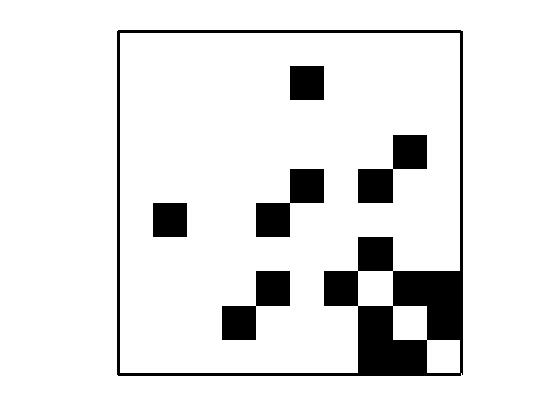
\includegraphics[width=0.225\textwidth]{\arraysfigsdir/adj.png}
      };
    \end{scope}
    \begin{scope}[xshift=0.08\textwidth]
      \node [mybox] (box){
        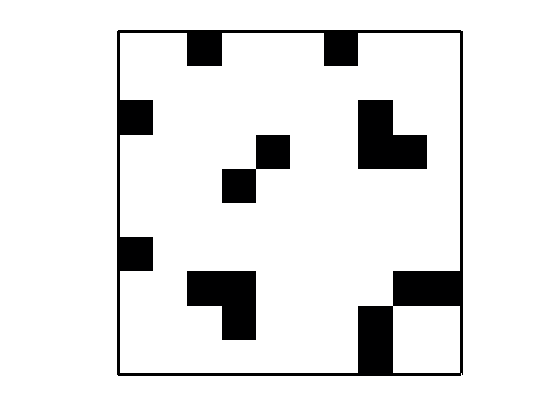
\includegraphics[width=0.225\textwidth]{\arraysfigsdir/adj_perm.png}
      };
    \end{scope}
    \begin{scope}[xshift=0.04\textwidth]
      \node[inner sep=0,text width=0.13\textwidth, text centered,font=\Huge] (note1) at (0,0) {
         $\equiv$};
    \end{scope}
  \end{scope}
\end{tikzpicture}

\end{tabular}
\caption{Left: Networks with equivalent structure but different node labels. Right: Corresponding adjacency matrix representations of these networks}
\label{fig:exchangeable}
\end{figure}

Relational data are typically stored in arrays; the right hand side of figure~\ref{fig:exchangeable} shows the corresponding adjacency matrix representations of the networks on the left.
We demonstrate that exchangeability of the objects underlying a relational database can be expressed in terms of array exchangeability.
Prior work on array exchangeability, both theoretical \citep[e.g.][]{Hoover1979, Aldous1981a, Hoover1982, Kallenberg1999a, Diaconis2007, Aldous2010, Austin2012, Choi2012, Wolfe2013} and applied \citep[e.g.][]{Hoff2007a,Roy2009,Lloyd2012}, has focused on single exchangaeble arrays.
We show that the representation theorems for single arrays can be used to derive representations for collections of exchangeable arrays \ie exchangeable databases.

\section{Exchangeable databases}

We abstractly define a database following the entity-relationship formalism \citep[e.g.][]{Ullman2002} where the values of attributes are the result of evaluating functions (relations) over a collection of entities / objects.

\newcommand{\bi}{\bm{i}}
\newcommand{\Types}{T}
\newcommand{\Space}{S}
\begin{definition}[types, signatures, relation]
Fix a finite set $\Types$ of \defn{types}.  Define a \defn{signature} to be a finite sequence $s \in \Types^d$ of types.
Define a \defn{relation $r$ of signature $s \in \Types^d$ with values in a space $\Space$} to be a function from $\Nats^d$ to $\Space$.
\end{definition}

We may encode a relation $r$ with signature $s \in \Types^d$ as an array $X^r \defas (X^r_{\bi})_{\bi \in \Nats^d}$ given by
\[
X^r_{\bi} = r(i_1,\dotsc,i_d), \qquad \text{for } \bi = (i_1,\dotsc, i_d) \in \Nats^d.
\]

\begin{example} 
Let $\Types = \{\textit{users,movies}\}$.
A relation $r$ of signature $(\textit{users},\textit{movies})$ taking values in $\{1,2,3,4,5\}$ might store movie ratings with rows corresponding to some enumeration of \textit{users}, and columns corresponding to some enumeration of \textit{movies}. 
A relation $r'$ of signature $(\textit{users},\textit{users})$ taking values in $\{0,1\}$ might store the symmetric friendship relations in a social network.
\end{example}

\begin{definition}[database]
Define a \defn{database} to be a collection of $R$ relations $r_1,\dotsc,r_R$ of signature $s_1,\dotsc,s_R$, respectively, taking values in $\Space_1,\dotsc,\Space_R$, respectively.
\end{definition}

We may encode a database as a collection of arrays $(X^{r_j})_{j=1}^R$, where $X^{r_j}$ encodes the relation $r_j$.  
For notational simplicity, we will often refer to the collection of arrays $(X^{r_j})_{j=1}^R$ as if it were the database itself.
%For notational simplicity, we will sometimes write $(X^r)$ to denote such a collection of arrays.

Permuting the ordering of objects within a database results in a permutation of the indices of several of the arrays encoding its relations.
For each type $t \in \Types$, let $p_t \in \SGinf$ be a permutation of $\Nats$. 
Write $p = (p_t ; t \in \Types) \in \SGinf^T$ for the collection of such permutations.
Given a signature $s \in \Types^d$, define $p^s$ to be the map from $\Nats^d$ to $\Nats^d$ such that
\[
p^s(\bi) \defas (p_{s_1}(i_1), \dotsc,p_{s_d}(i_d)), \qquad \text{for } \bi \in \Nats^d.
\]
In other words, $p^s$ maps a sequence $i_1,\dotsc,i_d$ of indices (indexing objects of type $s_1,\dotsc,s_d$, respectively) to the sequence where each index is permuted by the permutation corresponding to its type.

If $X^r$ is the encoding of a relation $r$ with signature $s \in \Types^d$, then the permuted relation $r \circ p$ is represented by the array $X^{r\circ p}$ given by
\[
X^{r \circ p}_{\bi} = X^r_{p^s(\bi)}, \qquad \text{for } \bi \in \Nats^d.
\]

%The permutation of a database $(X^r)$ by $p$ is simply the database $(X^r \circ p)$.

\begin{definition}[exchangeable database]
We say that a random database $(X^{r_j})_{j=1}^R$ is \emph{exchangeable} when it has the same distribution as $(X^{r_j\circ p})_{j=1}^R$ for every $p \in \SGinf^T$.
\end{definition}

%If the ordering of all objects is arbitrary, then $X^r$ is $\pi$-exchangeable where $\pi$ is the partition of consecutive integers with lengths $m^r_1, m^r_2, \ldots, m^r_O$.

%\PROBLEM{Here}

%Let $\Law(Y)$ be the law (distribution) of a random variable $Y$ and define $\chi_m X \defas (X_{i_1\ldots i_d}; \ i_j \le m )$.

The following result characterises the distribution of any exchangeable database to arbitrary accuracy.

\begin{cor}[functional representation for exchangeable databases]
  \label{cor:simple-database}
   Let $(X^{r_j})_{j=1}^R$ be an exchangeable random database.
   Then there exists a sequence of random measurable functions $F^{j,1}, F^{j,2}, \dotsc$ for 
   every $j=1\ldots R$ and collection of \iid Uniform$[0,1]$ random variables $(\AHvar^t_i)_{i\in\Nats,t \in \Types}$ such that 
   the random databases $(X^{r_j,n})_{j=1}^R$
    converge in distribution to $(X^{r_j})_{j=1\ldots R}$ as $mn\to \infty$, where   
%   the sequence of arrays $X^{j,1},X^{j,2},\dotsc$, for $j \in \{1,\dotsc,R\}$, given by
   \[
     X^{r_j,n}_{\bi} := F^{j,n}(\AHvar^{s_j(1)}_{i_1},\dotsc,\AHvar^{s_j(d)}_{i_d}), \qquad \text{for } \bi \in \Nats^d.
   \]
\end{cor}

This is a corollary of theorem~\ref{thm:simple-database} proven in section~\ref{sec:proof_database} which states that the law of fixed subarrays are mutually absolutely continuous and the associated Radon-Nikodym derivatives converge uniformly to $1$ as $n \to \infty$.
We also present an almost-sure representational result which requires some heavy notation which we build up in subsequent sections.

To demonstrate this theorem, we present two special cases of this result applicable to modelling a network with side information for each node and a social network with associated user-item data.

\begin{cor}
  \label{cor:network-side-simple}
  Consider an exchangeable database with one object type, one unary relationship, and one binary relationship; denote the binary relationship by the array $X=(X_{i,j})_{i,j\in\Nats}$ and the unary relationship with the sequence $C=(C_i)_{i\in\Nats}$.
   Then there exists a sequence of pairs of random measurable functions $(F^n, G^n)_{n\in\Nats}$ and a collection of \iid Uniform$[0,1]$ random variables $(\AHvar_{i})_{i\in\Nats}$ such that if we define the arrays $X^1,X^2,\dotsc$ and sequences $C^1,C^2,\dotsc$ by
   \[ 
     X^n_{i,j} &\defas F^n(\AHvar_{i},\AHvar_{j}), \qquad \text{for } i,j,n\in\Nats, \\
     C^n_{i} &\defas G^n(\AHvar_{i}), \qquad \text{for } i,n\in\Nats,
    \]
   then $(X^n,C^n)$ converges in distribution to $(X,C)$ as $n \to \infty$.
\end{cor}

\begin{cor}
  Consider an exchangeable database with two object types, one binary relation between two objects of the first type and a binary relation between objects of different types;  denote the first relation by the array $X=(X_{i,j})_{i,j\in\Nats}$ and the second by $Y=(Y_{i,k})_{i,k\in\Nats}$.
   Then there exists a sequence of pairs of random measurable functions $(F^n, G^n)_{n\in\Nats}$ and a collection of \iid Uniform$[0,1]$ random variables $(\AHvar_{i})_{i\in\Nats}, (\AHvaralt_{i})_{i\in\Nats}$ such that if we define the arrays $X^1,X^2,\dotsc$ and  $Y^1,Y^2,\dotsc$ by
   \[ 
     X^n_{i,j} &\defas F^n(\AHvar_{i},\AHvar_{j}), \qquad \text{for } i,j,n\in\Nats, \\
     Y^n_{i,k} &\defas G^n(\AHvar_{i}, \AHvaralt_{k}), \qquad \text{for } i,k,n\in\Nats,
    \]
   then $(X^n,Y^n)$ converges in distribution to $(X,Y)$ as $n \to \infty$.
\end{cor}

\begin{rem}[uniform distributions]\label{rem:uniform}
The uniform distributions in the theorem are canonical but the theorem still holds with any non-atomic probability measure on a Borel space \eg Gaussian distributions.
\end{rem}

\begin{rem}[random functions]\label{rem:randfunc}
\TBD{Explain precisely what is meant by a random function}
\end{rem}

\subsection{Intepretation and examples}

Corollary~\ref{for:simple-database} states that the joint distribution of an exchangeable database can be arbitrarily well approximated by a collection of random measurable functions and uniform random variables.
This functional form provides a set of parameters to be estimated that are naturally hierarchical.
The functions $(F^{j,n})$ capture properties of entire relations whilst the $(U^t_i)$ represent randomness associated with particular objects underlying the relational data.

\subsubsection{Example : Exchangeable networks}

Consider modeling a single binary relation which indicates whether or not two nodes in a network are connected or not.
This data is typically represented in the form of an adjacency matrix $(X_{ij})$ where $X_{ij} = 1$ if and only if node $i$ is connected to node $j$.
Theorem~\ref{thm:simple-database} states that if the distribution of $X$ is exchanegable then it can be arbitrarily well approximated by
\begin{equation}
(F(\AHvar_i, \AHvar_j))
\end{equation}
where $F$ is a random measurable function and $(U_i)$ are \iid Uniform$[0,1]$ random variables.
This special case has been used previously by \cite{Hoff2007a,Roy2009,Lloyd2012} to inspire probabilistic models of networks of the form
\begin{eqnarray}
(\AHvar_i) & \simiid & \textrm{\eg Gaussian} \\
F & \sim & \textrm{\eg Gaussian process, bilinear function}\ldots \\
W_{ij} & := & F(\AHvar_i, \AHvar_j) \\
X_{ij} | W_{ij} & \sim & \textrm{Bernoulli}(\sigma(W_{ij}))\label{eq:graphon}.
\end{eqnarray}
This is demonstrated pictorially in figure~\ref{fig:graphon}; in this case $F$ can be interpreted as a blurred adjacency matrix.

\begin{figure}[ht]
\centering
\begin{tabular}{c}
\begin{tikzpicture}[>=stealth,scale=0.0075\columnwidth]%,transform canvas={xshift=-3cm,yshift=1cm}]
  \begin{scope}[yshift=0.5cm]
  \begin{scope}
    \node [mybox] (box) at (0.5, -0.5){
    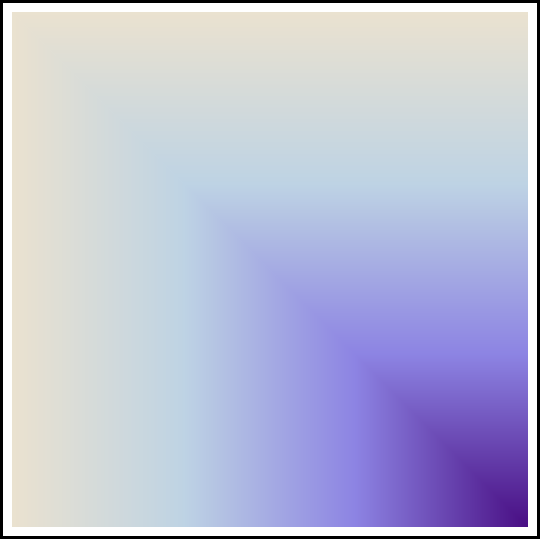
\includegraphics[width=0.225\columnwidth]{\arraysfigsdir/min_function.pdf} 
    };
    %\path[use as bounding box] (-0.5,0.5) rectangle (2.8,-1.5);
    %\draw (0,0) --(0,-1) --(1,-1) --(1,0) --(0,0);
    %\draw (0,0)--(1,-1);
    \node[font=\normalsize] at (0,0.1) {$0$};
    \node[font=\normalsize] at (-0.1,0) {$0$};
    \node[font=\normalsize] at (1,-1.1) {$1$};
    \node[font=\normalsize] at (1.1,-1) {$1$};
    \draw [dashed] (0.2,0.1) -- (0.2,-1.1); \node at (0.2,0.2) {$U_1$};
    \draw [dashed] (-0.1,-0.2) -- (1.1,-0.2); \node at (-0.25,-0.2) {$U_1$};
    \draw [dashed] (0.65,0.1) -- (0.65,-1.1); \node at (0.65,0.2) {$U_2$};
    \draw [dashed] (-0.1,-0.65) -- (1.1,-0.65); \node at (-0.25,-0.65) {$U_2$};
    \node[circle,fill,scale=0.4,color=red] at (0.65,-0.2) {};
  \end{scope}
  \begin{scope}[xshift=2cm]
    \draw (0,0)--(0,-1);
    \draw (-0.05,0)--(0.05,0); \node at (0.15,0) {$0$};
    \draw (-0.05,-1)--(0.05,-1); \node at (0.15,-1) {$1$};
    \node[circle,fill,scale=0.4,color=red] at (0,-0.21) {};
    \node[font=\normalsize] at (0.45,-0.23) {$\mbox{Pr}\lbrace X_{12}=1\rbrace$};
  \end{scope}
  \begin{scope}
  \draw[->] (0.7,-0.25) .. controls (1.3,-0.5) and (1.5,-0.5) .. (1.95,-0.26);
  \draw (1.4,-0.45) node [fill=white] {$\sigma(\Theta)$};
  \end{scope}
  \end{scope}
  %\begin{scope}[xshift=3.4cm]
  %  \node [mybox] (box){
  %  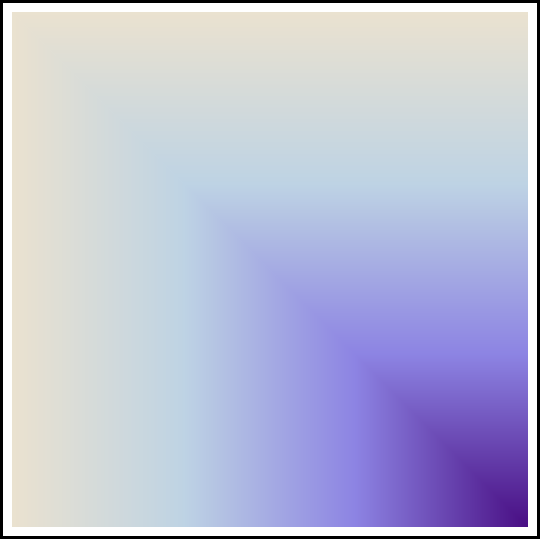
\includegraphics[width=0.18\columnwidth]{\arraysfigsdir/min_function.pdf} 
    %
\includegraphics[width=2.9cm]{\arraysfigsdir/uniform_attachment_graphon.pdf}
  %};
  %\end{scope}  
  %\begin{scope}[xshift=3.4cm]
  \begin{scope}[xshift=-1.2cm]
    \node [mybox] (box){
    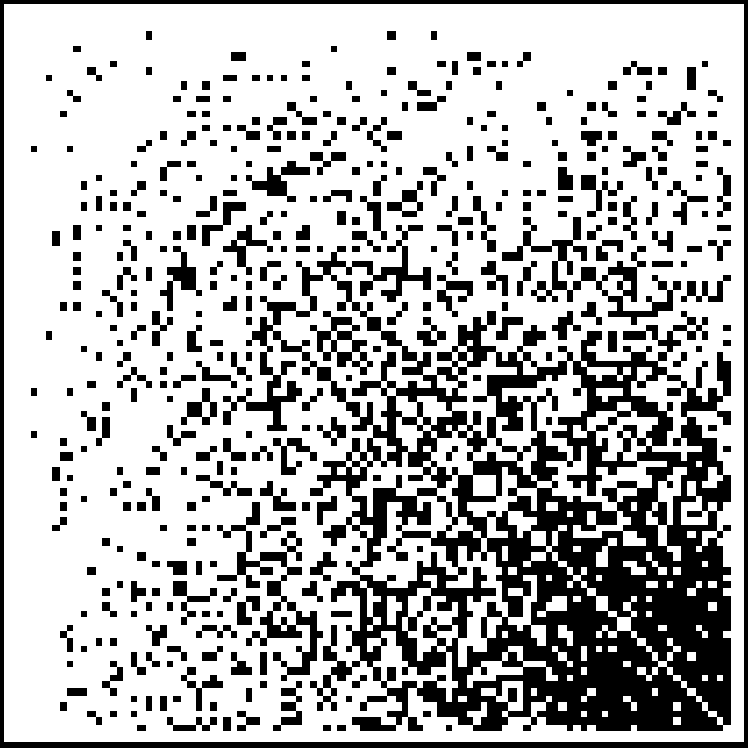
\includegraphics[width=0.225\columnwidth]{\arraysfigsdir/lovasz_sample100.pdf}
    %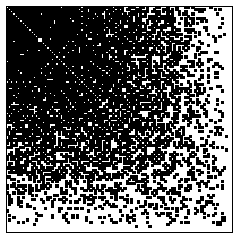
\includegraphics[width=2.8cm]{\arraysfigsdir/uniform_attachment_empirical.pdf}
  };
  \end{scope}
\end{tikzpicture}

\end{tabular}
\caption{
A pictorial representation of a model for network data inspired by the Aldous--Hover representation theorem.
The left shows a random sample of a binary network (represented by an adjacency matrix) generated by a model of the form given by equation~\eqref{eq:graphon}.
}
\label{fig:graphon}
\end{figure}

\subsubsection{Example : A simple database}

Consider the simple database shown on the left hand side of figure~\ref{fig:multi-rel-seq}.
There are two objects, students and courses, and three relations, the unary relation `age' acting on students, the binary relation `friends' acting on pairs of students and the binary relation `grade' that acts on students and courses.
Sample data encoded in arrays is shown at the bottom of this figure.

Exchangeability of this database means that the entries of the leftmost table, the rows and columns of the second table and the rows of the third table can be arbitrarily permuted without changing the distribution of the database when viewed as a random variable.
Similarly the columns of the rightmost table may be independently arbitrarily permuted.

The functional form resulting from the application of theorem~\ref{thm:simple-database} to this data structure is shown on the right hand side of figure~\ref{fig:multi-rel-seq}.
The two objects are represented by \iid random variables, $(U_i)$ for students, $(V_i)$ for courses and the three relations are represented by three random functions $F(\AHvar_i),G(\AHvar_i,\AHvar_j)$ and $H(\AHvar_i,\AHvaralt_j)$ whose inputs are the random variables representing the objects the relations act upon.

\begin{figure}[ht]
\centering
\begin{tabular}{cc}
\tiny \begin{tikzpicture}[scale=0.5, node distance = 4cm, auto]
  % Define block styles
  \tikzstyle{decision} = [diamond, draw, fill=blue!20, 
      text width=4.0em, text badly centered, node distance=1.0cm, inner sep=0pt]
  \tikzstyle{invisible} = [diamond, draw=white, fill=white, 
      text width=4.0em, text badly centered, node distance=1.0cm, inner sep=0pt]
  \tikzstyle{block} = [rectangle, draw, fill=blue!20, 
      text width=4.0em, text centered, rounded corners, minimum height=2em]
  \tikzstyle{placeholder} = [rectangle, draw, 
      text width=5em, text centered, rounded corners, minimum height=2em]
  \tikzstyle{line} = [draw, -latex']
  \tikzstyle{cloud} = [draw, ellipse,fill=red!20, node distance=0.75cm,
      minimum height=1em]
  \begin{scope}[yshift=0cm]
    % Place nodes
    \node [block] (student) at (-2.5,1) {Student};
    %\node [block, right of=student] (course) {Course};
    \node [block] (course) at (+2.5,1) {Course};
    \node [decision] at(+2.5, -1.5) (takes) {Takes};
    \node [cloud] (friends) at (-2.5, -4.0) {Friends};
    \node [cloud] (grade) at (+2.5, -4.0) {Grade};
    \node [cloud] (age) at (-5.5, -4.0) {Age};
    % Draw edges
    \path [line] (student) -- (takes);
    \path [line] (course) -- (takes);
    \path [line] (takes) -- (grade);
    %\path [line] (student) -- (observed);
    %\path [line] (observed) -- (friends);
    \draw[->] (student.south) .. controls (-1.0,-1) and (-1.0,-2) .. (friends.north east);
    \draw[->] (student.south) .. controls (-4.0,-1) and (-4.0,-2) .. (friends.north west);
    \path [line] (student.south west) -- (age.north east);
  \end{scope}
  \begin{scope}[yshift=-5cm]
    \draw (-4,0) --(-4,-3) --(-1,-3) --(-1,0) --(-4,0);
    \draw (0,0) --(0,-3) --(5,-3) --(5,0) --(0,0);
    \draw (-6.5,0) --(-6.5,-3) --(-4.5,-3) --(-4.5,0) --(-6.5,0);
    \draw (0,0) --(0,-3) --(5,-3) --(5,0) --(0,0);
    \node at (-3.25, -0.25) {\checkmark};
    \node at (-2.75, -0.25) {\checkmark};
    \node at (-2.25, -0.25) {\checkmark};
    \node at (-1.75, -0.25) {\checkmark};
    \node at (-1.25, -0.25) {\checkmark};
    \node at (-3.75, -0.75) {\checkmark};
    \node at (-3.75, -1.25) {\checkmark};
    \node at (-3.75, -1.75) {\checkmark};
    \node at (-3.75, -2.25) {\checkmark};
    \node at (-3.75, -2.75) {\checkmark};
    \node at (-2.75, -0.75) {$\times$};
    \node at (-3.25, -1.25) {$\times$};
    \node at (-1.25, -1.75) {\checkmark};
    \node at (-2.25, -2.75) {\checkmark};
    
    \node at (0.25, -0.25) {A};
    \node at (4.25, -0.75) {A};
    \node at (3.75, -1.25) {B};
    \node at (1.25, -2.75) {B};
    \node at (0.75, -1.25) {C};
    \node at (2.75, -2.75) {C};
    \node at (2.25, -1.25) {D};
    \node at (2.25, -1.75) {D};
    \node at (3.75, -0.75) {E};
    \node at (4.75, -1.25) {F};
    
    \node at (-5.5, -0.25) {15};
    \node at (-5.5, -0.75) {15};
    \node at (-5.5, -1.25) {15};
    \node at (-5.5, -1.75) {14};
    \node at (-5.5, -2.25) {14};
    \node at (-5.5, -2.75) {16};
  \end{scope}
\end{tikzpicture}
 & \tiny \begin{tikzpicture}[scale=0.5, node distance = 4cm, auto]
  % Define block styles
  \tikzstyle{decision} = [diamond, draw, fill=blue!20, 
      text width=4.0em, text badly centered, node distance=1.0cm, inner sep=0pt]
  \tikzstyle{block} = [rectangle, draw, fill=blue!20, 
      text width=4.0em, text centered, rounded corners, minimum height=2em]
  \tikzstyle{placeholder} = [rectangle, draw, 
      text width=5em, text centered, rounded corners, minimum height=2em]
  \tikzstyle{line} = [draw, -latex']
  \tikzstyle{cloud} = [draw, ellipse,fill=red!20, node distance=0.75cm,
      minimum height=1em]
  \begin{scope}[yshift=0cm]
    % Place nodes
    \node [block] (student) at (-2.5,0) {$(\AHvar_i)$};
    %\node [block, right of=student] (course) {Course};
    \node [block] (course) at (+2.5,0) {$(\AHvaralt_i)$};
    \node [decision, below of=student] (observed) {Observed};
    \node [decision, below of=course] (takes) {Takes};
    \node [cloud] (friends) at (-2.5, -4.0) {Friends};
    \node [cloud] (grade) at (+2.5, -4.0) {Grade};
    \node [cloud] (age) at (-5.5, -4.0) {Age};
    % Draw edges
    \path [line] (student) -- (takes);
    \path [line] (course) -- (takes);
    \path [line] (takes) -- (grade);
    %\path [line] (student) -- (observed);
    \path [line] (observed) -- (friends);
    \draw[->] (student.south) .. controls (-2.0,-0.8) and (-2.0,-1.0) .. (observed.north east);
    \draw[->] (student.south) .. controls (-3.0,-0.8) and (-3.0,-1.0) .. (observed.north west);
    \path [line] (student.south west) -- (age.north east);
  \end{scope}
  \begin{scope}[yshift=-5cm]
    \draw (-4,0) --(-4,-3) --(-1,-3) --(-1,0) --(-4,0);
    \draw (0,0) --(0,-3) --(5,-3) --(5,0) --(0,0);
    \draw (-6.5,0) --(-6.5,-3) --(-4.5,-3) --(-4.5,0) --(-6.5,0);
    \draw (0,0) --(0,-3) --(5,-3) --(5,0) --(0,0);
%    \node at (-3.25, -0.25) {\checkmark};
%    \node at (-2.75, -0.25) {\checkmark};
%    \node at (-2.25, -0.25) {\checkmark};
%    \node at (-1.75, -0.25) {\checkmark};
%    \node at (-1.25, -0.25) {\checkmark};
%    \node at (-3.75, -0.75) {\checkmark};
%    \node at (-3.75, -1.25) {\checkmark};
%    \node at (-3.75, -1.75) {\checkmark};
%    \node at (-3.75, -2.25) {\checkmark};
%    \node at (-3.75, -2.75) {\checkmark};
%    \node at (-2.75, -0.75) {$\times$};
%    \node at (-3.25, -1.25) {$\times$};
%    \node at (-1.25, -1.75) {\checkmark};
%    \node at (-2.25, -2.75) {\checkmark};
    \node at (-2.5, -1.5) {$(G(\AHvar_i, \AHvar_j))$};
    
%    \node at (0.25, -0.25) {A};
%    \node at (4.25, -0.75) {A};
%    \node at (3.75, -1.25) {B};
%    \node at (1.25, -2.75) {B};
%    \node at (0.75, -1.25) {C};
%    \node at (2.75, -2.75) {C};
%    \node at (2.25, -1.25) {D};
%    \node at (2.25, -1.75) {D};
%    \node at (3.75, -0.75) {E};
%    \node at (4.75, -1.25) {F};
    \node at (2.5, -1.5) {$(H(\AHvar_i, \AHvaralt_j))$};
    
%    \node at (-5.5, -0.25) {15};
%    \node at (-5.5, -0.75) {15};
%    \node at (-5.5, -1.25) {15};
%    \node at (-5.5, -1.75) {14};
%    \node at (-5.5, -2.25) {14};
%    \node at (-5.5, -2.75) {16};
    \node at (-5.5, -1.5) {$(F(\AHvar_i))$};
  \end{scope}
\end{tikzpicture}

\end{tabular}
\caption{Left: A pictorial representation of a relational database. Right: The functional representation of the distribution of data of this form guaranteed to be an arbitrarily good approximation by theorem~\ref{thm:simple-database}}
\label{fig:multi-rel-seq}
\end{figure}

\section{Proof of exchangeable database representation theorem}
\label{sec:proof_database}

\subsection{Background: $\pi$-exchangeability}

This section reviews material from \TBD{cite Kallenberg}.

Let $\pi$ be a partition of the set $\{1,\dots,d\}$ and $p = \{p^{\pi_i} : i = 1,\dots,d\}$ be a collection of permutations of $\Nats$ where $\pi_i \defas \{I \in \pi : i \in I\}$.
We say that an array $X^r$ representing relation $r$ is $\pi$-exchangeable if 
\begin{equation}
  X^{r\circ p} \eqd X
\end{equation}
for all collections $p$ of permutations of $\Nats^d$ of the form given above.
Note that this is precisely the type of symmetry we encountered for exchangeable databases.

We say that a $\pi$-exchangeable array $X$ is simple if it admits a functional representation of the form
\begin{equation}
  X_{\bi} = F(U, U^{\pi_1}_{\bi_1}, \dots, U^{\pi_d}_{\bi_d})
\end{equation}
where $F$ is a measurable function and $U, U^{\pi_j}_{\bi_j}$ are \iid Uniform$[0,1]$ random variables.

\begin{prop}[Borel hypercube]
  \label{prop:hypercube}
  Result about encoding arbitrarily many random variables with functions and a uniform random variable
\end{prop}

\begin{thm}[$\pi$-exchangeability representation theorem]
  \label{thm:piex}
  Let $X$ be a $\pi$-exchangeable array.
  Then there exist some simple $\pi$-exchangeable arrays $X_1$ , $X_2$ , \dots such that
  $\Law(\chi_m X_n) \sim \Law(\chi_m X)$ for all $m,n \in \Nats$ and the associated densities tend
  uniformly to 1 as $n \to \infty$ for fixed $m$.
\end{thm}

where $\Law$ represents the distribution or law of a random variable, $X \sim Y$ indicates that the distributions $X$ and $Y$ are mutually absolutely continuous and $\chi_m$ is the array subset operation such that $\chi_m X \defas \{X_{\bi} : \bi \in \{1,\dots,m\}^d\}$.

We say that an exchangeable database $(X^{r_j})_{j=1}^R$ is simple if it admits a functional representation of the form
\begin{equation}
  X^{r_j}_{\bi} = F^{r_j}(U, U^{s_{j}(1)}_{\bi_1},\dots,U^{s_{j}(d_j)}_{\bi_{d_j}}) \,\, \forall \,\, \bi \in \Nats^{d_j} \,\, \forall \,\, j \in {1,\dots,R}.
\end{equation}

We can now state and prove the simple database representation theorem.

\begin{thm}[Simple exchangeable database representation theorem]
  \label{thm:simple-database}
  Let $(X^{r_j})_{j=1}^R$ be an exchangeable database.
  Then there exist some simple exchangeable databases $(X^{r_j,1})_{j=1}^R$ , $(X^{r_j,2})_{j=1}^R$ , \dots such that
  $\Law(\chi_m (X^{r_j,n})_{j=1}^R) \sim \Law(\chi_m (X^{r_j})_{j=1}^R)$ for all $m,n \in \Nats$ and the associated densities tend
  uniformly to 1 as $n \to \infty$ for fixed $m$.
\end{thm}

\begin{proof}
  Each array $(X^{r_j})$ is $\pi$-exchangeable where $\pi$ is given by the blocks of $\{1,\dots,n_j\}$ whose signature have the same type.
  We can therefore apply theorem~\ref{thm:piex} to each array separately resulting in representations
\begin{equation}
  G^{r_j,n}(U^j,U^{s_{j}(1),j}_{\bi_1},\dots,U^{s_{j}(d_j),j}_{\bi_{d_j}})
\end{equation}
We tie these representation together by applying proposition~\ref{prop:hypercube} to the collections of uniforms $(U^{t,j}_{\bi})_{j=1}^R$, encoding them as a single uniform random variable
\begin{equation}
  U^t_{i} = H^t(U^{t,1}_{i},\dots,U^{t,R}_{i})
\end{equation}
where $H^t$ is bi-measurable and similarly for $U = H^t(U^{1},\dots,U^{R})$.
Notice that $U_{\bi}, U^t_{\bi}$ are independent by construction.
We now define functions
\begin{equation}
F^{r_j,n}(U,U^{s_{j}(1)}_{\bi_1},\dots,U^{s_{j}(d_j)}_{\bi_{d_j}}) = G^{r_j,n}(U^j,U^{s_{j}(1),j}_{\bi_1},\dots,U^{s_{j}(d_j),j}_{\bi_{d_j}})
\end{equation}
which are measurable by the measurability of $G$ and $H$.
We are now essentially done.
\end{proof}

\begin{rem}[simpler proof mechanisms that do not work]
\label{rem:randfunc}
\NA{
The above proof mechanism is somewhat concise and feels a little bit non-constuctive when invoking the Borel hypercube isomorphism theorem.
}
\end{rem}

\section{An almost sure representation theorem}
\label{sec:almost_sure}

To prove an almost sure representational theorem will require some considerably more difficult notation.
We have followed the notation in \NA{Kallenberg} but we have adapted it to try to make it easier to understand.
However, there is only so much we can do so we provide corollaries of the theorem after its statement and proof to demonstrate that behind the notation are some fairly simple concepts.
Brace yourself.

We define for each $k \in \Nats^d$ and $I \subset \{1,\ldots,d\}$ a set $k_I \subset \Nats$ by
\begin{equation}
k_I = \{k_i: i \in I\}, \quad k \in \Nats^d
\end{equation}
\ie $k_I$ only includes certain indices.

We further define $k_{\pi I}$ by
\begin{equation}
  k_{\pi I} = (k_{I \cap J} : J \in \pi)
\end{equation}
N.B. we have replaced Kallenberg's function notation with a list since this may be more natural to the readers of this work.
Let $\Nats^{\leq d}$ be the collection of all subsets of the naturals $K \subset \Nats$ with cardinality $|K| \leq d$.

\begin{prop}[\citet{Kallenberg1999-pj}]
\label{prop:piexas}
  Let $X$ be a random $d$-array in a Borel space $S$.
  Then $X$ is $\pi$-exchangeable iff there exists a measurable function $f:[0,1]^{2^d}\to S$ and a $U$-array $\xi$ with index set $\prod_{J\in\pi} \Nats^{\leq |J|}$ such that
  \begin{equation}
    X_k = f(\xi_{k_{\pi I}} : I \subset \{1,\ldots,d\}) \ \as, \quad k \in \Nats^d.
    \label{eq:piexas}
  \end{equation}
\end{prop}

We now extend this theorem to the case of an exchangeable database.
We will spend some time defining notation specific to a particular exchangeable database; the proof will then follow concisely.

Start with an exchangeable database $(X^{r_j})_{j=1}^R$.
Assume w.l.o.g.\ that the types are ordered (\eg type 1, type 2,\dots) and the types in each signature respect this ordering (\eg $s = (1,1,2,3,3,\dots)$).
Define the multiplicity of a type $t$ in signature $s$ by the number of times the type appears in the signature, and denote this by $m_{t}^s$.
Define the maximum multiplicity of a type $t$ in a database as $m_t = \max_j m_t^{s_j}$.
Let $d = \sum_{t\in T} m_t$ be the sum of the multiplicities.
Let $d_j = \sum_{t\in T} m_t^s$ be the sum of the multiplicities for a particular signature.
Let $\pi$ be the partition of $\{1,\ldots,d\}$ consisting of consecutive blocks of integers with sizes equal to $\{m_1,\ldots,m_T\}$.
For a signature $s$ let $I_s$ be the subset of $\{1,\ldots,d\}$ that contains the first $m_1^s$ integers and then not the next $m_1 - m_1^s$ integers, then the next $m_2^s$ integers, and then not the next $m_2 - m_2^s$ integers and so on.
Finally, let $\mathbb{I}_s$ be the indicator function of the set $I_s$ within $\{1,\ldots,d\}$ and let $k^s \defas (k_i : i \in I_s)$.
Let $\pi_s \defas \{J \cap I_s : J \in \pi\}$

\begin{thm}[almost sure functional representation for exchangeable databases]
  \label{thm:as-database}
  A database $(X^{r_j})_{j=1}^R$ is exchangeable iff there exist measurable functions $f^j : [0,1]^{2^{d_j}} \to S_j$ such that
  \begin{equation}
    X_{k^{s_j}}^{r_j} = f^j(\xi_{k_{\pi I}} : I \subset I_{s_j}) \ \as, \quad k \in \Nats^d, \ j \in \{1,\ldots,R\}.
  \end{equation}
\end{thm}

\begin{proof}
Collections of arrays with this functional form are trivially exchangeable databases, so we include only the proof that exchangeable databases have this functional form.
Each array $X^{r_j}$ in an exchangeable database is $\pi_{s_j}$-exchangeable by definition.
Therefore, by proposition~\ref{prop:piexas} we have an almost sure representation
\begin{equation}
  X^{r_j}_{k^{s_j}} = g^j(\xi^j_{k_{\pi_{s_j} I}} : I \subset I_{s_j}) \ \as, \quad k \in \Nats^d
\end{equation}
Note this is exactly equation~\ref{eq:piexas} but with $\{1,\dots,d\}$ replaced by $I_{s_j}$.
Trivially, we can replace the $\pi_{s_j}$ in the previous expression with $\pi$ alone.
We now invoke proposition~\ref{prop:hypercube} to recode our $U$-array
\begin{equation}
  \xi_{\bi} = h((\xi^j_{\bi})_{j=1}^R) \,\, \forall \,\, \bi \in \prod_{J\in\pi} \Nats^{\leq |J|}
\end{equation} 
and then we just define some new measurable functions
\begin{equation}
  f^j(\xi_{k_{\pi_{s_j} I}} : I \subset I_{s_j}) = g^j(\xi^j_{k_{\pi_{s_j} I}} : I \subset I_{s_j}) \ \as, \quad k \in \Nats^d
\end{equation}
and we are essentially done.
\end{proof}

\subsection{Examples}

\begin{cor}
  Consider an exchangeable database with one object type, one unary relationship, and one binary relationship; denote the binary relationship by the array $X=(X_{i,j})_{i,j\in\Nats}$ and the unary relationship with the sequence $C=(C_i)_{i\in\Nats}$.
   Then there exist measurable functions $(F, G)$ and a collection of \iid Uniform$[0,1]$ random variables $U, (\AHvar_{i})_{i\in\Nats}, (\AHvar_{\{i,j\}})_{i,j\in\Nats}$ such that
   \[ 
     X_{ij} & = F(U, \AHvar_{i},\AHvar_{j}, \AHvar_{\{i,j\}}), \qquad \text{for } i,j,n\in\Nats, \\
     C_i & = G(U, \AHvar_{i}), \qquad \text{for } i,n\in\Nats,
    \]
almost surely.
\end{cor}

That is, this is the Aldous--Hoover representation for a jointly exchangeable array and the DeFinetti representation of an exchangeable sequence at the same time, with coupled uniform random variables.

\begin{cor}
  Consider an exchangeable database with two object types, one binary relation between two objects of the first type and a binary relation between objects of different types;  denote the first relation by the array $X=(X_{i,j})_{i,j\in\Nats}$ and the second by $Y=(Y_{i,k})_{i,k\in\Nats}$.
   Then there exists a pair of measurable functions $(F, G)$ and a collection of \iid Uniform$[0,1]$ random variables $U, (\AHvar_{i})_{i\in\Nats}, (\AHvaralt_{i})_{i\in\Nats}, (\AHvar_{\{i,j\}})_{i,j\in\Nats}, (W_{i,j})_{i,j\in\Nats}$ such that
   \[ 
     X_{ij} & = F(U,\AHvar_{i},\AHvar_{j},  \AHvar_{\{i,j\}}),  \qquad &\text{for } i,j\in\Nats, \\
     Y_{ik} & = G(U, \AHvar_{i}, \AHvaralt_{k}, W_{ik}), \qquad &\text{for } i,k\in\Nats,
    \]
almost surely.
\end{cor}

That is, this is the Aldous--Hoover representation for a jointly exchangeable array and the Aldous--Hoover representation of a separately exchangeable array at the same time, but with coupled uniform random variables due to the shared objects underlying the data.

\begin{cor}
  Consider an exchangeable database with two object types, one binary relation between two objects of the first type and a ternary relation between two objects of the first type and one of the type;  denote the first relation by the array $X=(X_{i,j})_{i,j\in\Nats}$ and the second by $Y=(Y_{i,j,k})_{i,j,k\in\Nats}$.
   Then there exists a pair of measurable functions $(F, G)$ and a collection of \iid Uniform$[0,1]$ random variables $U, (\AHvar_{i})_{i\in\Nats}, (\AHvaralt_{i})_{i\in\Nats}, (\AHvar_{\{i,j\}})_{i,j\in\Nats}, (W_{i,j})_{i,j\in\Nats} (Z_{\{i,j\}k})_{i,j,k\in\Nats}$ such that
   \[ 
     X_{ij} & = F(U,\AHvar_{i},\AHvar_{j},  \AHvar_{\{i,j\}}),  \qquad &\text{for } i,j\in\Nats, \\
     Y_{ijk} & = G(U, \AHvar_{i}, U_j \AHvaralt_{k}, \AHvar_{\{i,j\}}, W_{ik}, W_{jk}, Z_{\{i,j\},k}), \qquad &\text{for } i,j,k\in\Nats,
    \]
almost surely.
\end{cor}

That is, this is the Aldous--Hoover representation for a jointly exchangeable array and the Kallenberg representation of a $\pi$-exchangeable array at the same time, but with coupled uniform random variables due to the shared objects underlying the data.

\section{A generic statistical model template}

In analogy to the work of \cite{Hoff2007-ja, Roy2009-ge, Lloyd2012-sb} on exchangeable arrays, theorem~\ref{thm:simple-database} naturally inspires a generic generative model of exchangeable databases.
Each object of type $t$ in the database is associated with an \iid sample, $\AHvar_i^t$, from some distribution $\mathcal{U}$ \eg Uniform, Gaussian.
For each relation $r_1,\dotsc,r_R$ we sample a random function $F^j$ from some distribution $\mathcal{F}^j$, \eg Gaussian process, random (bi/tri/\ldots)linear functions.
We denote the evaluation of these functions at the corresponding values of $(\AHvar_i^t)$ by $W^j$.
$W^j$ can then be passed through a link function and distribution $L^j(\cdot)$ to model the observed value of the relation $r_j$.
\[
(\AHvar_i^t) & \simiid  \mathcal{U} \\
F^j & \sim  \mathcal{F}^j \\
W^j_{\bi} & \defas F^j(\AHvar^{s_j(1)}_{i_1},\cdots,\AHvar^{s_j(n)}_{i_n}) \\
X^{r_j}_{\bi} \given W & \sim  L^j(W^j_{\bi}) \qquad \text{independently across $j$ and $\bi$.}
\]

\begin{rem}[dependence between functions]
In general, the functions $F^j$ may be dependent.
However, the representation results presented in this chapter provide no guidance on the form of this dependence; stronger assumptions than exchangeability would have to be made.
In practice one may model the functions to be independent a priori at the risk of wasting statistical strength.
\end{rem}

\subsection{Discriminative models as well}

Consider the representation result for a social network with side information on each user presented in corollary~\ref{cor:network-side-simple}. The natural generative model for such data inspired by the is representation is
\[
  U_i & \simiid \mathcal{U} \\
  F & \sim \mathcal{F} \\
  G & \sim \mathcal{G} \\
  X_{ij} & \sim L^X(F(U_i, U_j)) \\
  C_{i} & \sim L^C(G(U_i))
\]
but in the situation where $C$ is fully observed and the task is to predict missing entries of $X$ it may be unnecessary to learn a model of $C$.
Indeed, if $C$ is assumed to be noiselessly observed, then we have $C_i = L^C(G(U_i))$ where $L^C(G(.))$ is a deterministic function.
We can then choose to model $X$ as follows
\[
  F'(U_i, U_j, C_i, C_j) & = F'(U_i, U_j, L^C(G(U_i)), L^C(G(U_j))) = F(U_i, U_j) \\
  X_{ij} & \sim L^X(F'(U_i, U_j, C_i, C_j)).
\]
Furthermore we could choose $F'$ to not depend on $U_i, U_j$ resulting in the model
\[
  X_{ij} & \sim L^X(F''(C_i, C_j))
\]
which is simply a regression model.

Indeed, the same logic can be applied to applied to exchangeable sequences to derive more standard regression models.
Suppose that $(X_i, Y_i)$ is an exchangeable sequence.
By DeFinetti's theorem we can model this as
\[
  U_i & \sim \mathcal{U} \\
  F & \sim \mathcal{F} \\
  G & \sim \mathcal{G} \\
  X_i & \sim L^X(F(U_i)) \\
  Y_i & \sim L^Y(G(U_i))
\]
and by similar arguments to those above, if we were to assume that $X$ was noiselessly observed we could model $Y$ as
\[
  Y_i & \sim L^Y(G(X_i))
\]
which is a standard regression model, or
\[
  Y_i & \sim L^Y(G(U_i, X_i))
\]
which is halfway between latent variable modelling and regression.
An example of this model structure can be found in \cite{Wang2012-rc} but is otherwise surprisingly uncommon.

Now suppose we perfectly observe a binary relation; what can this tell us about modelling a related unary relation?
We now demonstrate how we could reconstruct an example model presented in \cite{Friedman1999-mo}.
They present a simple genetic model where one's maternal chromosome depends on your mother's maternal and paternal chromosomes and similarly for one's paternal chromosome.
In this example we have two binary relations, mother-of and father-of and two unary relations, maternal and paternal chromosomes.
We write this as $X_{ij} = 1 \iff$ person $i$ is the mother of person $j$ and $Y_{ij} = 1 \iff$ person $i$ is the father of person $j$\fTBD{Change this to case notation to show that it is zero otherwise}.
Further let $M_i$ and $P_i$ be the maternal and paternal chromosomes of person $i$ respectively.
A potential form of a model for this data is
\[
  U_i & \sim \mathcal{U} \\
  F & \sim \mathcal{F} \\
  G & \sim \mathcal{G} \\
  H & \sim \mathcal{H} \\
  J & \sim \mathcal{J} \\
  X_{ij} & \sim L^X(F(U_i, U_j)) \\
  Y_{ij} & \sim L^Y(G(U_i, U_j)) \\
  M_i & \sim L^M(H(U_i)) \\
  P_i & \sim L^P(J(U_i))
\]
Applying similar arguments to before we can replace $U_i$ by $U_i'  \defas (U_i, V_i, M_i, P_i)$.
We could then define
\begin{align}
L^X(F(U_i',U_j')) &= 
  \begin{cases}
    1 & \textrm{if } (M_i, P_i) = U_j \\
    0 & \textrm{otherwise}  
  \end{cases}\\
L^Y(G(U_i',U_j')) &=
  \begin{cases}
    1 & \textrm{if } (M_i, P_i) = V_j \\
    0 & \textrm{otherwise}  
  \end{cases}
\end{align}
Performing inference in this model we would then find that in the posterior $U_i = (M_j, P_j)$ where person $j$ is the mother of person $i$ and similarly for $V_i$.
This would then allow the functions $H$ and $J$ to specify that the maternal chromosome of person $i$ depend probabilistically on the chromosomes of their mother and similarly for their paternal chromosome.
We have therefore shown how this particular probabilistic relational model can be cast in the form guaranteed to exist by the theorems presented in this chapter.
In principle, suitable prior distributions on the latent variables and functions could learn such a representation purely from data, although in this situation it is sensible to use prior knowledge.

However, the canny reader will have noticed that the functions $L^X(F(.,.))$ and $L^Y(G(.,.))$ defined above are almost everywhere zero.
This is exactly because the relations mother-of and father-of define sparse graphs with in-degrees of at most one.
As remarked before\TBD(reference), any not almost everywhere zero representing function will imply density when modelling a graph.
The above exercise is certainly quite a contortion that is only clear when one knows the model one is aiming at.
General representation results for sparse graphs that can usefully imply model structures are still unknown.

\NA{
All this suggests to me that we should try an observed and latent hybrid model of some sort.
I wonder to what extent this has been attempted?
The idea would be that all objects have some latent variables attached to them that can explain features of objects, noisy relations of objects and features or noisy relations of related objects.
Yes, the learning PRMs paper suggests this and has a handful of references but says it is in general an interesting problem without remarking much on how it might look in real life - actually the references just consider entirely hidden nodes.
However, \cite{Menon2011-ku} considers using both side information and latent factors for matrix factorisation.
}

\subsection{Higher order dependencies}

So far we have only considered probabilistic models inspired by the simple array versions of exchangeability theorems.
Do the almost sure representation theorems with their more detailed latent variable representations tell us anything?
Consider the following dataset: we have a social network $X_{ij}$ and a ternary relation $Y_{ijk}$ that records if both person $i$ and person $j$ have been to location $k$.
The simple array inspired representation of this data is of the form
\[
  X_{ij} & \sim L^X(F(U_i, U_j)) \\
  Y_{ijk} & \sim L^Y(G(U_i, U_j, V_k))
\]
and in contrast the almost sure result would a more elaborate model of the form
\[
  X_{ij} & \sim L^X(F(U_i, U_j, U_{\{ij\}})) \\
  Y_{ijk} & \sim L^Y(G(U_i, U_j, U_{\{ij\}}, V_k, W_{ik}, W_{jk}, Z_{\{ij\}k})).
\]
Now suppose that $X$ included information on the type of relations in the social network, and that people $i$ and $j$ were in a romantic relationship.
This knowledge would make it more likely for this couple to visit \eg restaurants typically frequented by couples.
In the almost sure representation this information could easily be transferred from $X$ to the modelling of $Y$ via the shared latent variable $U_{\{i,j\}}$.
In the simple array representation this knowledge would somehow have to be encoded in the latent variables $U_i$ and $U_j$ meaning that the problem of sharing this information is at least as hard as producing an effective generative model of which pairs of people are in a relationship which could be difficult given limited information.

I am however unaware of any standard probabilistic models making use of this type of dependence.
This is most probably due to the potentially large computational barrier to storing and inferring the values of latent variables for each pair of objects.
There may however be use in this type of relationship on small datasets where one can afford relatively high computational costs to perform a more detailed analysis of a dataset.

\subsection{A brief word about longitudinal data}

We won't say much not the matter, but it is worth mentioning how all of the modelling paradigms presented here can be extended to longitudinal data (\ie time varying).
For example, consider longitudinal measurements of a social network $X_{ij}^t$.
Let $Y_{ij} \defas \{X_{ij}^t : t \in \mathcal{T}\}$ where $\mathcal{T}$ represents some period of time.
Then $Y_{ij}$ can be assumed to be exchangeable meaning that we can represent its distribution as
\[
  Y_{ij} = G(U_i, U_j)
\]
which in turn means
\[
  X_{ij}^t = G^t(U_i, U_j)
\]
or more conventionally
\[
  X_{ij}^t = F(U_i, U_j, t)
\]
meaning that we can represent the distribution of the time evolving social network with fixed latent variables for each node but a time varying representing function.
The form of the time varying function is completely general, but it could be constrained further by assumptions of continuity, Markov assumptions or Markov exchangeability for example.
It is more typical however to assume that the latent variables also evolve through time (this still produces an exchangeable distribution) with the representing function potentially static.
\TBD{
Mention that only the functions need vary in time, but typically it makes life easier if the latent variables also get to change in time.
Reference Ryan Adams basketball work and Dunson's work on this.
}
It may be advantageous however to have fixed latent variables when one is jointly modelling both time evolving and static data.

\subsection{Prior work using models of this form}

Don't forget this early block model variant \cite{Hoffman_undated-ri}.

In section~\ref{sec:networks:related} it was demonstrated that many models of single 2-arrays fit the form of the generic model presented above.
In particular there are models that assume $F$ is linear \citep[e.g.][]{Hoff2007a, Meeds2007, Salakhutdinov2008, Yu2008, Miller2009}, that $F$ is Gaussian process distributed \citep[e.g.][]{Lawrence2009, Yan2011, Lloyd2012} and other non-linear forms for $F$ both parametric \citep[e.g.][]{Hoff2002} and nonparametric \citep[e.g.][]{Roy2009}.
In addition to this there has been a line of work that uses increasingly more expressive forms of the distribution $\mathcal{U}$ \citep[e.g.][]{Wang1987, Nowicki2001, Kemp2006, Xu2006, Meeds2007, Miller2009, Palla2012}.

Many, but not all, of these models have been extended to model $d$-arrays.
A summary of models using linear forms of $F$ is given in \cite{Kolda2009-ba}; non-linear models include \cite{Xu2012} (cite the latest inftucker stuff).

For full databases, the literature is limited to clustering / block / latent class models \cite{Kemp2006} \TBD{don't forget IHRM} and models using linear forms for the $F^r$ \citep[e.g.][]{Acar, Acar2012, Acar2013, Andersen2013, Davison, Ermis1958, Gallinari2011, Jimeng2009, Kong2010, Lippert2008, Networks, Nickel2011, Shangguan2012, Singh, Singha, Singh2008}.

We should certainly expect to see new research using some of the more advanced forms proposed for networks being applied to higher order arrays or full databases.
However, rather than proposing yet more specific models it would be very interesting to see automated model building techniques applied to these domains, potentially combined with model forms inspired by probabilistic relational models.

\section{Discussion}

We have demonstrated how the concept of exchangeability can be applied to databases and used to derive a natural parameter space for statistical models of such data.
Identifying a parameter space is the first step in any statistical analysis, allowing either frequentist estimation of the parameters or Bayesian prior specification.
This concept is well established for exchanegable sequences where de Finetti's theorem \citep[e.g.][]{Kallenberg2005} applies.
For exchangeable arrays, the relevant representation theorems were presented by Aldous and Hoover \cite{Aldous1981a, Hoover1979} over 30 years ago but it is only recently that these results are being used to inspire Bayesian models \cite{Hoff2007a, Roy2009, Lloyd2012} and frequentist estimation procedures \cite{Kallenberg1999a,Choi2012, Wolfe2013}.
We hope that this work will continue and be extended to the analysis of exchangeable databases.

\subsection{Mention sparsity again}

\TBD{This is really important to talk about at all times!}

\outbpdocument{
\bibliographystyle{plainnat}
\bibliography{references.bib}
}
